\section{Instrument Signature Removal for DP2 Science Data} \label{sec:isr-science}

Figure~\ref{fig:isr-pipeline} lists the ISR correction tasks in the order they are applied to science images for DP2.
This section integrates the calibration products described in \S\ref{sec:calibration-production} and summarizes how they compose during routine science processing.
Corrections are applied in reverse chronological order relative to the photon transfer chain (\S\ref{sec:processing:detector-physics} and Figure~\ref{fig:detector-boxes}).

\begin{figure*}[t]
    \centering
    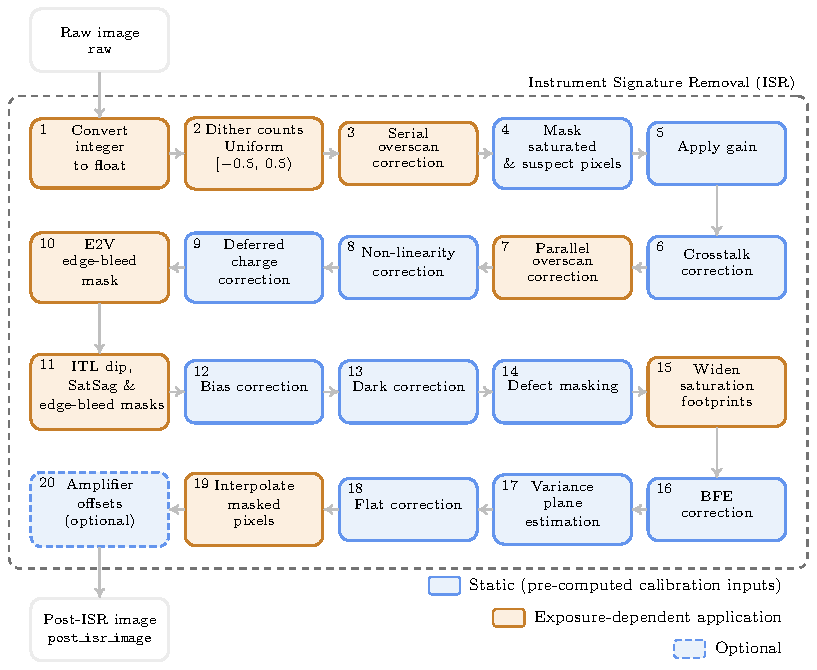
\includegraphics[width=0.9\textwidth]{figures/isr-pipeline.pdf}
    \caption{Outline of the Instrument Signature Removal Pipeline (ISR) applied to LSSTCam science images for DP2.
    The steps in the pipeline follow a very specific sequence determined by the physics of the instrument signature and where it enters in the photon transfer chain.}
    \label{fig:isr-pipeline}
\end{figure*}

\subsection{ISR Pipeline Overview} \label{sec:isr-science:overview}

The following outline follows Figure~\ref{fig:isr-pipeline} step by step.
Each item names the ISR task, the calibration product applied, and the subsection in \S\ref{sec:calibration-production} where that product is derived.
% TODO: Replace placeholder step names with labels from Figure~\ref{fig:isr-pipeline}.

\begin{itemize}
    \item \textbf{[ISR step name].}
    Calibration product: [product name].
    See \S\ref{sec:processing:calibration:curated-calibs} / \S\ref{sec:processing:calibration:auxiliary-data-products} / \S\ref{sec:processing:calibration:xtalk} / \S\ref{sec:processing:calibration:defects} / \S\ref{sec:processing:calibration:linearity} / \S\ref{sec:processing:calibration:cti} / \S\ref{sec:processing:calibration:ptc} / \S\ref{sec:processing:calibration:bf} / \S\ref{sec:processing:calibration:bias} / \S\ref{sec:processing:calibration:dark} / \S\ref{sec:processing:calibration:flats} as appropriate.
    \item \textbf{[ISR step name].}
    Calibration product: [product name].
    See the corresponding subsection in \S\ref{sec:calibration-production}.
    % Repeat for each step in Figure~\ref{fig:isr-pipeline}.
\end{itemize}

\subsection{Intermediate and Bootstrap ISR Passes} \label{sec:isr-science:bootstrap}

Some calibration production paths require intermediate ISR passes that do not correspond to the final science ISR sequence shown in Figure~\ref{fig:isr-pipeline}.
\begin{itemize}
    \item Deferred-charge (CTI) calibration applies an intermediate ISR pass with defect masking and non-linearity correction before EPER measurement (\S\ref{sec:processing:calibration:cti}).
    \item CTI and PTC calibration production share a bootstrap cycle: a temporary, non-CTI-corrected PTC supplies initial per-amplifier gains for CTI calibration inputs, after which a fully CTI-corrected PTC is fit for science ISR (\S\ref{sec:processing:calibration:cti}, \S\ref{sec:processing:calibration:ptc}).
\end{itemize}
% TODO: Document any additional intermediate passes (e.g., pre-PTC linearity or defect-only passes) once the dependency graph is finalized.

\subsection{Curated Calibrations and Header Provenance} \label{sec:isr-science:provenance}

Describe how curated calibration collections are selected and attached to science exposures for DP2 processing.
Header metadata records which ISR steps were applied and which calibration dataset versions were used; see \S\ref{sec:verify-accept-certify:data-products} for the verification and distribution context.
% TODO: Cross-reference curated-calibration bundle contents (\S\ref{sec:processing:calibration:curated-calibs}) and auxiliary products (\S\ref{sec:processing:calibration:auxiliary-data-products}).
